\section*{Operazioni utili}
\addcontentsline{toc}{section}{Operazioni utili} 
\rhead{Operazioni utili}

\subsection*{Variabili d'ambiente}
\addcontentsline{toc}{subsection}{Variabili d'ambiente} 
Per il corretto funzionamento del tool devono essere configurate correttamente le variabili d'ambiente di sistema. In particolar modo, bisogna aggiungere alla variabile 'PATH' i seguenti valori:
\begin{itemize}[nosep]
\item[-] \textbf{Emulator} C:\textbackslash Users\textbackslash User\textbackslash AppData\textbackslash Local\textbackslash Android\textbackslash Sdk\textbackslash Emulator
\item[-] \textbf{platform-tools} C:\textbackslash Users\textbackslash User\textbackslash AppData\textbackslash Local\textbackslash Android\textbackslash Sdk\textbackslash platform-tools 
\item[-] \textbf{build-tools} C:\textbackslash Users\textbackslash User\textbackslash AppData\textbackslash Local\textbackslash Android\textbackslash Sdk\textbackslash build-tools\textbackslash 31.0.0
\end{itemize}
\noindent I percorsi potrebbe variare in base alle scelte effettuate in fase di installazione di Android Studio.



\subsection*{Migrazione del progetto ad AndroidX}
\addcontentsline{toc}{subsection}{Migrazione del progetto ad AndroidX} 
AndroidX è un'importante miglioramento della libreria di supporto Android originale, che non viene più mantenuta. I pacchetti AndroidX sostituiscono completamente la libreria di supporto fornendo parità di funzionalità e nuove librerie. \newline
La migrazione del progetto ad AndroidX può essere facilmente effettuata seguendo la guida ufficiale (\url{https://developer.android.com/jetpack/androidx/migrate}). In caso si incontrino dei problemi/errori, può essere di aiuto la risorsa 'Migrating to AndroidX: Tip, Tricks, and Guidance' (\url{https://medium.com/androiddevelopers/migrating-to-androidx-tip-tricks-and-guidance-88d5de238876}).

\subsection*{Registrazione del caso di test con Espresso Test Recorder}
\addcontentsline{toc}{subsection}{Registrazione del caso di test con Espresso Test Recorder} 

Espresso Test Recorder è uno strumento già integrato all’interno di Android Studio che permette la registrazione automatica dei casi di test[5]. Dopo aver caricato il progetto in AS, basterà avviare il tool cliccando sulla voce 'Record Espresso Test' nel menù 'Run'.  Lo strumento registra automaticamente (utilizzando la libreria Espresso) le operazioni effettuate sull'emulatore che sarà avviato.  Espresso Test Recorder permette inoltre di aggiungere delle asserzioni. La Figura \ref{fig:record.esempio} mostra un istantanea effettuata durante la registrazione del caso di test utilizzando lo strumento.
\begin{figure}[H]
	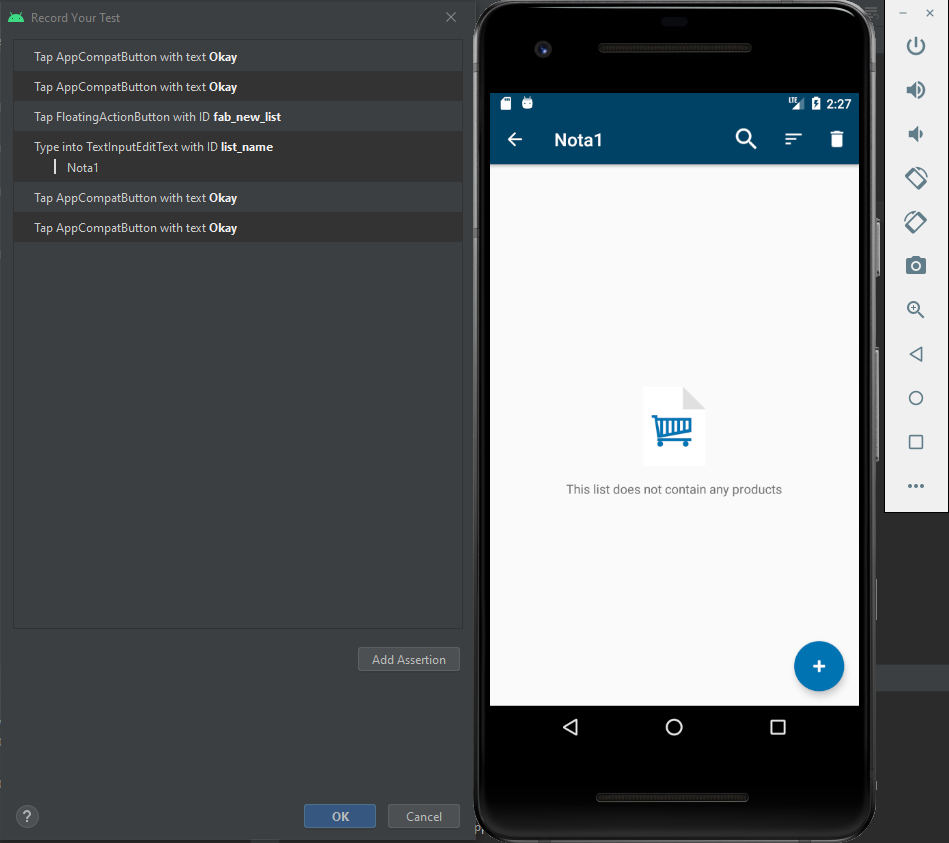
\includegraphics[scale=0.35]{record.esempio}
	\centering
	\caption{Espresso Test Recorder}
    \label{fig:record.esempio}
\end{figure}

\subsection*{Generazione degli APK in Android Studio}
\addcontentsline{toc}{subsection}{Generazione degli APK in Android Studio}

Android Studio offre un comando che genera automaticamente l'APK di test e l'APK dell'applicazione. Per utilizzalo basterà scegliere nella barra del menu:
\begin{itemize} [nosep]
\item [] Build -> Build Bundle(s) / APK(s) -> Build APK(s)
\end{itemize}
Prima di utilizzare il comando, è necessario controllare la configurazione delle Build variant del progetto (File -> Project structure -> BuildVariants). In particolar modo, nella build variant che ci interessa (solitamente 'debug'), bisogna controllare che i campi Application ID Suffix e Version Name Suffix siano vuoti e in caso contrario cancellare il contenuto. 


\subsection*{Configurazione degli AVD}
\addcontentsline{toc}{subsection}{Configurazione degli AVD} 
Gli AVD possono essere configurati lanciando lo strumento 'AVD Manager' (Appendice A - AVD Manager) direttamente da Android Studio. Nell'interfaccia di avvio di Android Studio (Figura \ref{fig:avd1}), basta cliccare sui 3 puntini in alto a destra e, nel menu a tendina, selezionare 'AVD Manager'. Dalla schermata che si apre (Figura \ref{fig:avd2}) possono essere facilmente creati e gestiti gli emulatori. Il nome di ogni emulatore nel file di configurazione generale deve corrispondere con il nome di uno degli AVD in questa schermata. Il tool non è in grado di gestire gli AVD creati con spazi nel nome.

\begin{figure}[H]
    \centering
    \begin{minipage}{0.4\textwidth}
        \centering
        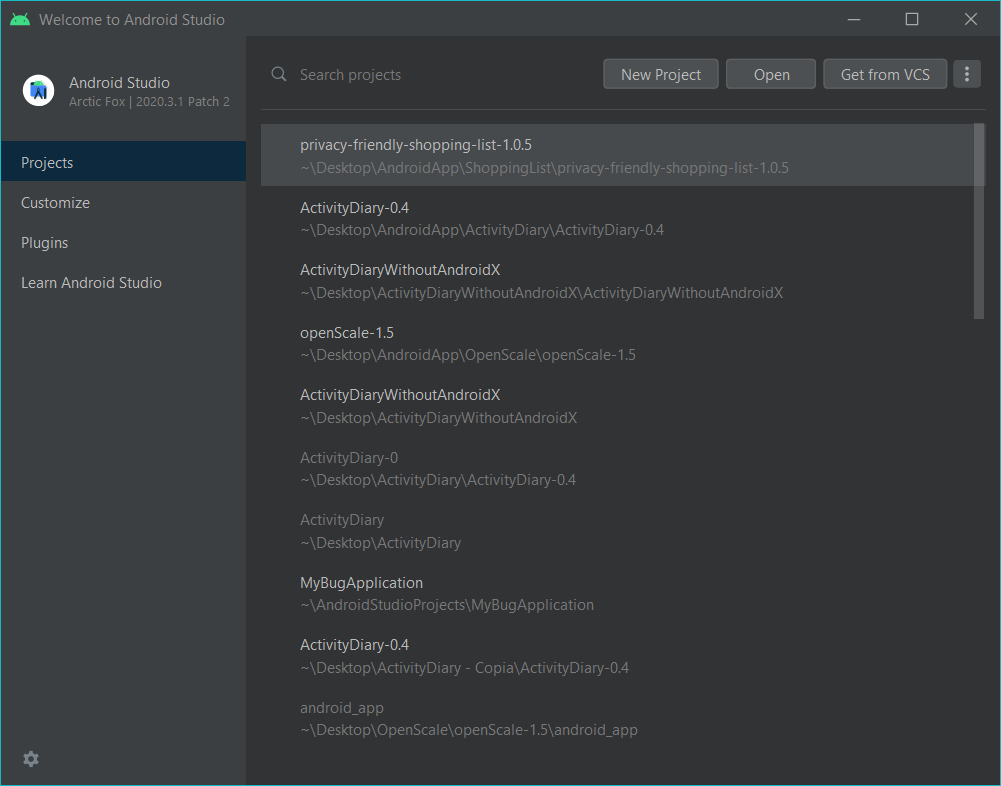
\includegraphics[width=7cm]{avd.1} 
        \caption{Schermata iniziale AS}
            \label{fig:avd1}
    \end{minipage}\hfill
    \begin{minipage}{0.6\textwidth}
        \centering
        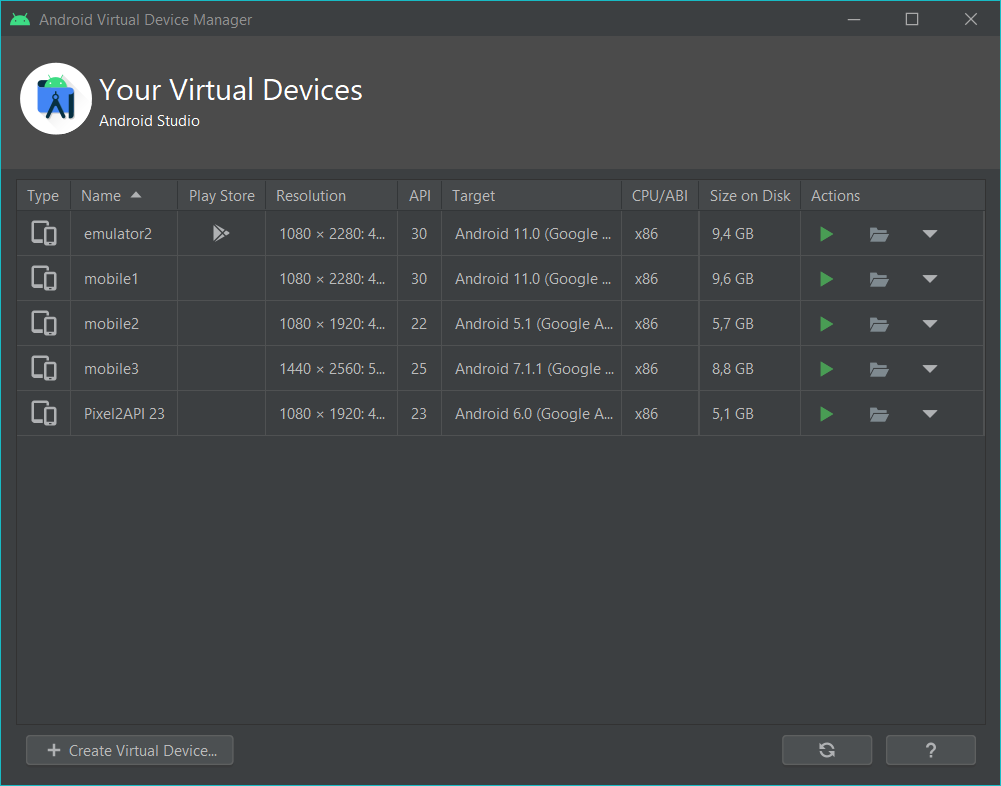
\includegraphics[width=7cm]{avd.2} 
        \caption{Schermata iniziale AVD Manager}
            \label{fig:avd2}
    \end{minipage}\hfill
\end{figure}





\subsection*{Lettura degli alberi xml}
\addcontentsline{toc}{subsection}{Lettura degli alberi xml} 

\label{sect:xmltree}
In questa sezione vengono illustrate le tipologie di nodo/attributo utilizzate per la rappresentazione degli alberi xml nella relazione, in modo da garantirne una migliore comprensione. L'esposizione comprende una serie di esempi, che fanno riferimento all'albero in Figura \ref{fig:configstructure}.

\begin{itemize} [nosep]	
		\item \textbf{root element}  \newline
		Un nodo di tipo 'root element' può avere figli. Non possono coesistere nello stesso livello dell'albero più nodi di tipo 'root element' con lo stesso tag. \newline
		\textcolor{gray}{\emph{Esempio - Il nodo con tag 'Applications', in quanto di tipo 'root element', può avere figli , ma deve essere l'unico nodo con il tag 'Applications' nel livello dell'albero in cui si trova. Quindi il di configurazione dovrà avere, come figli di 'root' solo un nodo con tag 'Applications' e solo un nodo con tag 'Emulators'. Il nodo 'root' non può quindi avere, per esempio, più di un nodo figlio con tag 'Applications'.}}
		\item \textbf{element}  \newline
		Un nodo di tipo 'element' può avere figli. Possono coesistere nello stesso livello dell'albero più nodi di tipo 'element' con lo stesso tag. \newline
		\textcolor{gray}{\emph{Esempio - Il nodo 'Applications' può avere più figli con il tag 'Application' in quanto, essendo quest'ulimo di tipo 'element', è consentita la coesistenza di nodi con lo stesso tag nel medesimo livello dell'albero. Inoltre il tag 'Application', sempre per la sua tipologia, può avere dei nodi figli, in questo caso con tag 'Bug'.}}
		\item \textbf{empty element}  \newline
		Un nodo di tipo 'empty element' non può avere figli (nodo foglia). Possono coesistere nello stesso livello dell'albero più nodi di tipo 'empty element' con lo stesso tag. \newline
			\textcolor{gray}{\emph{Esempio - Il nodo 'Colums' può avere più figli con il tag 'Column' in quanto, essendo quest'ulimo di tipo 'empty element', è consentita la coesistenza di nodi con lo stesso tag nel medesimo livello dell'albero. Inoltre il tag 'Column', sempre per la sua tipologia, non può avere dei nodi figli'.}}
			\item \textbf{full element}  \newline
		Un nodo di tipo full element' non può avere figli (nodo foglia). Non possono coesistere nello stesso livello dell'albero più nodi di tipo 'full element' con lo stesso tag.
		\item \textbf{attribute}  \newline
		Ogni nodo può e deve avere come attributi solo gli attributi 'figli' rappresentati nell'albero. \newline
		\textcolor{gray}{\emph{Esempio - Il nodo 'Bug' può e deve avere come attributi 'id', ' type', 'description'.}}
\end{itemize}



\subsection*{Generazione degli APK}
\addcontentsline{toc}{subsection}{Generazione degli APK} 
\label{genapk}
%\lhead{Generazione degli APK}
La generazione dei file APK dell'applicazione (\emph{app.apk} nella relazione) e APK di test (\emph{test.apk} nella relazione), entrambi file di input per la funzionalità di automazione dei test, verrà affrontata nei seguenti passi:
\begin{itemize}[nosep]
\item [1.] Creazione della classe di test 
\item [2.] Parametrizzazione della classe di test
\item [3.] Generazione dei file APK
\end{itemize}
\noindent Al termine verrà dedicato un paragrafo (Generazione degli APK senza disporre del codice sorgente) alla generazione dei file APK nel caso in cui non si disponga del codice sorgente.

\subsubsection*{1.Creazione della classe di test}
\rhead{Creazione della classe di test}
\label{creazioneclassetest}
Il primo step da affrontare nella generazione degli APK riguarda la creazione della classe che contiene, come unico caso di test, il caso di test in grado di riprodurre il bug. Una volta aperto il progetto dell'applicazione in Android Studio (Appendice A - Android Studio), la classe può essere:
\begin{itemize}[nosep]
\item [$\blacksquare$]\textbf{scritta manualmente} \newline
Utilizzando la libreria Espresso (Appendice A - Espresso)
\item [$\blacksquare$]\textbf{registrata automaticamente} \newline
Utilizzando lo strumento, già integrato nell’editor, Espresso Test Recorder  (Appendice A - Espresso Test Recorder) (Appendice A - Registrazione del caso di test con Espresso Test Recorder) 
\end{itemize}
In ogni caso, la classe di test creata dovrà essere posizionata nella cartella "androidTest" (cartella generato automaticamente da Android Studio per contenere gli instrumented tests) visibile nella vista 'Android' di Android Studio (Figura \ref{fig:and.android.studio}).


\begin{figure}[H]
    \centering
    \begin{minipage}{0.4\textwidth}
        \centering
        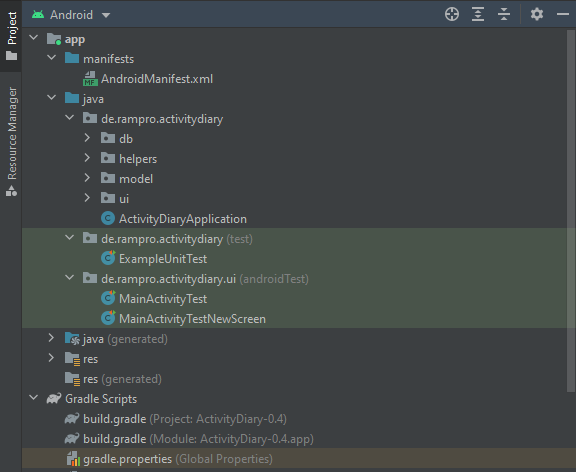
\includegraphics[scale=0.44]{and.android.studio} 
        \caption{Vista 'Android' in Android Studio - progetto 1}
            \label{fig:and.android.studio}
    \end{minipage}\hfill
    \begin{minipage}{0.5\textwidth}
        \centering
        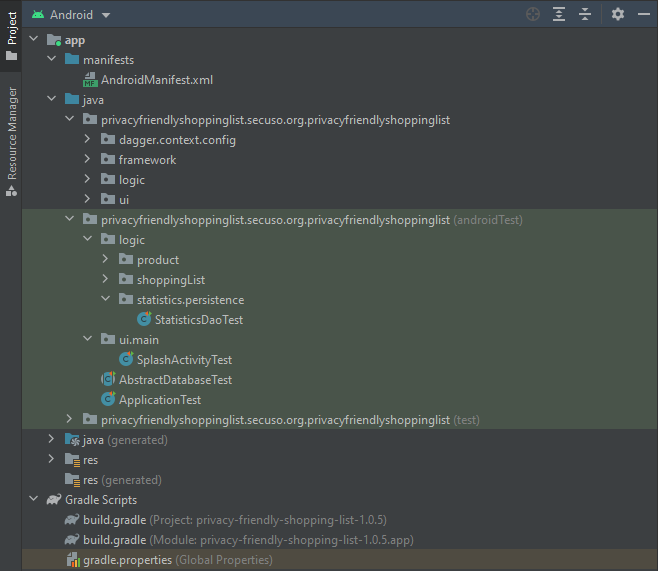
\includegraphics[scale=0.38]{and.2.android.studio} 
        \caption{Vista 'Android' in Android Studio - progetto 2}
            \label{fig:and.2.android.studio}
    \end{minipage}\hfill
\end{figure}

\bigskip
\noindent\textbf{Posizione della classe di test} \\
Il posizionamento della classe di test all'interno della cartella 'androidTest' influisce sul valore del parametro \emph{@class}, essenziale all'esecuzione della funzione di automazione dei test. In particolare:
\begin{itemize} [nosep]
\item [$\blacksquare$] \textbf{Caso 1} (consigliato) \newline
Nel caso in cui la classe sia posizionata nella radice (direttamente nella cartella 'androidTest'), il valore del parametro \emph{@class} dovrà semplicemente coincidere con il nome della classe di test.  \newline
\textcolor{gray}{Esempio - In Figura \ref{fig:and.android.studio}, nel caso in cui la classe contenente il caso di test che riproduce il bug sia 'MainActivityTest', il parametro \emph{@class} dovrà semplicemente assumere il valore 'MainActivityTest' }
\item [$\blacksquare$] \textbf{Caso 2} \newline
Nel caso in cui la classe sia posizionata in un package interno alla cartella 'androidTest', il valore del parametro \emph{@class} dovrà rispettare il pattern [pacchetto].[className] .  \newline
\textcolor{gray}{Esempio - In Figura \ref{fig:and.2.android.studio}, nel caso in cui la classe contenente il caso di test che riproduca il bug sia 'StatisticsDaoTest', il parametro \emph{@class} dovrà assumere il valore 'logic.statistics.persistence.StatisticsDaoTest' }
\end{itemize}

\subsubsection*{2.Parametrizzazione della classe di test}
\label{paramclasstest}
\rhead{Parametrizzazione della classe di test}
Il secondo step da affrontare nella generazione degli APK riguarda la parametrizzazione della classe di test di cui la creazione è stata affrontata nel punto precedente. Come analizzato nella Sezione \ref{pasparam}, nell'automazione dei test, per ogni lancio del test parametrico, i parametri vengono passati  alla strumentazione di test in formato JSON. Dalla classe di test si può avere accesso agli argomenti del bundle della strumentazione e quindi ai parametri di esecuzione.
\\\\
\noindent Per rendere la classe di test parametrica è necessario inserire, all'inizio di questa, il codice in Figura \ref{fig:parametrized};

\begin{figure}[H]
	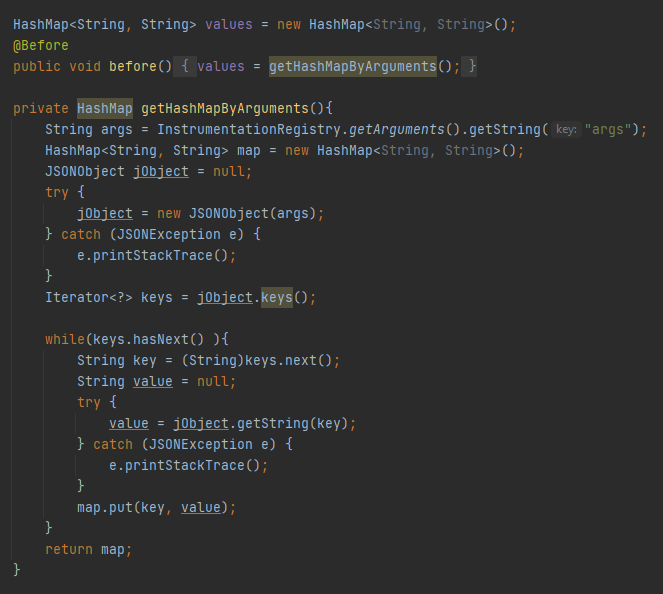
\includegraphics[scale=0.50]{parametrized}
	\centering
	\caption{Codice per la parametrizzazione delle classi di test}
    \label{fig:parametrized}
\end{figure}

\noindent Il funzionamento del codice, nel dettaglio, può essere sintetizzato come segue :
\begin{enumerate}[nosep]
\item dichiara e inizializza una hashmap (\emph{values});
\item prima di eseguire qualsiasi caso di test, assegna un nuovo valore alla struttura dati appena creata chiamando il metodo \emph{getHashMapByArguments()} che:
\begin{itemize} [nosep]
\item[1.] ottiene dalla strumentazione di test la stringa passata contenente i parametri in formato json;
\item[2.] dichiara e inizializza una nuova hasmap;
\item[3.] ricrea l'oggetto JSON dalla stringa ottenuta;
\item[4.] per ogni coppia chiave-valore dell'oggetto, aggiunge un elemento alla hasmap appena creata (con la stessa coppia chiave-valore);
\item[4.] ritorna l'hashmap;
\end{itemize}
\end{enumerate}
\bigskip
\noindent A questo punto, l'hasmpap \emph{values} contiene i parametri del test come coppia chiave-valore, in cui la chiave è rappresentata dall'etichetta della colonna del file di input a cui il valore fa riferimento. Si può quindi procedere alla parametrizzazione del caso di test in quanto l'hashmap \emph{values}  ha visibilità in tutta la classe.

\bigskip

\noindent Quindi, nei punti in cui il caso di test prevede l'inserimento di dati in input da parte dell'utente, il valore da inserire può essere ottenuto dall'hashmap specificando come chiave la colonna del file di input che contiene il dato  (\emph{values.get("inputColumnName")}). In Figura \ref{fig:esempio.parametrized} viene mostrato un esempio di parametrizzazione di un caso di test.

\begin{figure}[H]
	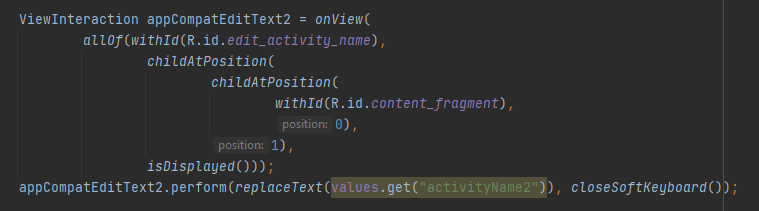
\includegraphics[scale=0.50]{esempio.parametrized}
	\centering
	\caption{Esempio: parametrizzazione della classe di test}
    \label{fig:esempio.parametrized}
\end{figure}

\subsubsection*{3.Generazione dei file APK}
\rhead{Generazione dei file APK}
L'ultimo step riguarda la vera e propria generazione dei file \emph{app.apk} e \emph{test.apk}. Android Studio è in grado di generare i file richiesti automaticamente grazie all'integrazione di Gradle (Appendice A - Generazione degli APK in Android Studio) (Appendice A - Gradle). Al termine della generazione dei file, nell'Event Log di AS viene comunicata la directory in cui questi sono stati creati.  Solitamente il file che nella relazione è chiamato \emph{app.apk} viene generato come \emph{app-debug.apk}, mentre il file che nella relazione è chiamato \emph{test.apk} viene generato come \emph{app-debug-androidTest.apk}.


\subsubsection*{Generazione degli APK senza disporre del codice sorgente}
\label{genapknocod}
\rhead{Generazione dei file APK senza disporre del codice sorgente}
Nei paragrafi precedenti è stata trattata la generazione degli APK supponendo di essere sempre in possesso del codice sorgente. In realtà, nella maggior parte dei casi, le applicazioni non sono open source e risulterebbe quindi utile poter utilizzare lo strumento anche nel caso in cui si disponga solamente dell'APK.  Il collega A. Mendieta, nella sua relazione di laurea triennale, ha trovato un metodo per la generazione dell'APK di test anche nel caso in cui non si possieda il codice sorgente (ma solo l'APK dell'applicazione), che ancora oggi è risultato utilizzabile.
\\\\
\noindent Brevemente, la soluzione individuata dal collega, utilizza un progetto open source (Appendice A - AndroidTestWithOutSource Project) che permette di generare solamente l'APK di test contenente la classe parametrizzata. In questo caso, la classe di test non può essere registrata con Espresso Test Recorder, ma deve essere scritta manualmente sfruttando le funzionalità offerte dallo strumento Ui Automator Viever (Appendice A - UI Automator Viewer). 
\\\\
\noindent Prima di poter utilizzare l'APK dell'applicazione e l'APK di test generata come file di input per il tool, risulta essenziale firmare gli APK con la stessa firma, operazioni facilmente effettuabile grazie allo strumento apksigner (Appendice A - apksigner).

